
\section{mpolishing.rb 一般グラフの研磨\label{sect:mpolishing}}

一般グラフデータに対して、データ研磨アルゴリズムを適用することで、
ノイズを除去し、グラフの濃淡をより鮮明にした「研磨グラフ」を生成する。
まずは、直感的な理解を得るために、図\ref{fig:polish0}と図\ref{fig:polish1}に研磨前のグラフと研磨後のグラフを示す。
オリジナルのグラフについて、濃い部分構造はより濃く、そして薄い部分構造はより薄くなるように研磨される。
結果として、中規模の極大クリーク(他の完全部分グラフに包含されない完全部分グラフ)が多く生成される。

\begin{figure}[htbp]
\begin{center}
\begin{tabular}{cc}

\begin{minipage}{0.3\hsize}
\begin{center}
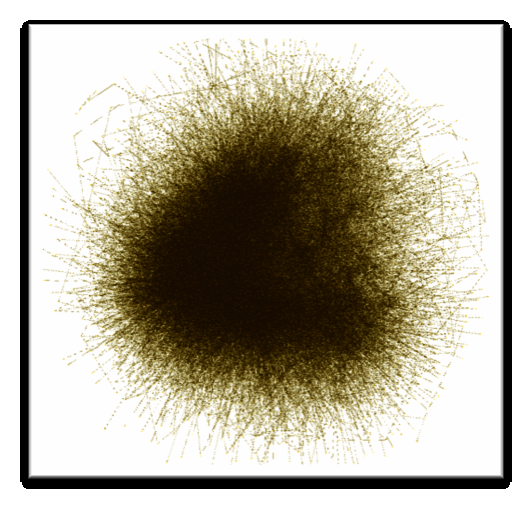
\includegraphics[scale=0.5]{./polish0.eps}
\caption{研磨前のグラフ\label{fig:polish0}}
\end{center}
\end{minipage}

\begin{minipage}{0.3\hsize}
\begin{center}
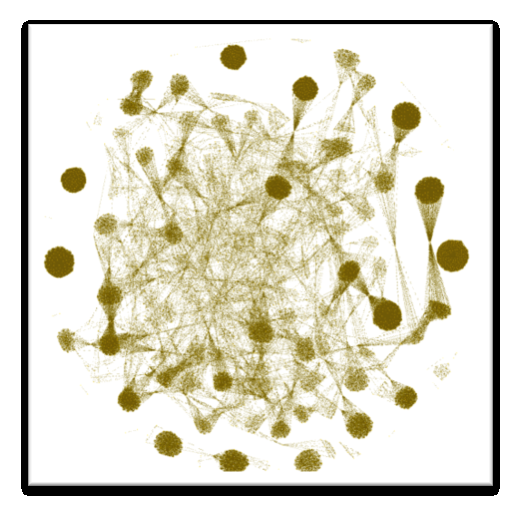
\includegraphics[scale=0.5]{./polish1.eps}
\caption{研磨後のグラフ\label{fig:polish1}}
\end{center}
\end{minipage}

\end{tabular} 
\end{center}
\end{figure} 

研磨のアルゴリズムをAlgorithm \ref{algo:polish}に示す。
ここに示されたアルゴリズムは、非常に効率の悪い方法ではあるが、理解のし易さを優先させている。
実際に内部で実装されているアルゴリズムについては参考文献\cite{Uno2014}に詳しい。
研磨の方法は至ってシンプルで、全ての頂点ペアについて、その類似度(後述)がユーザの指定した閾値以上であれば接続し、
そうでなければ接続しないというルールに従って、新たなグラフを再構成する。


\begin{algorithm}
\caption{グラフ研磨アルゴリズム\label{algo:polish}}
\begin{small}
\begin{algorithmic}[1]
\Function{Polishing}{$G=(V,E),\sigma$}
	\State $V:頂点集合, E:辺集合, \sigma: 類似度下限値$
	\State $E'=\phi$; $V'=\phi$ \Comment 研磨後の辺集合と頂点集合の初期化
	\ForAll{$u\in V$}
		\ForAll{$v\in V$} \Comment \# 全頂点ペア$u,v$について調べる
			\If{$sim(u,v)\ge\sigma$} \Comment 頂点ペア$u,v$が似ていればには新たに辺として加え、似てなければ加えない
				\State $E'=E'\cup (u,v)$
				\State $V'=V'\cup u$
				\State $V'=V'\cup v$
			\EndIf
		\EndFor
	\EndFor
	\State {\bf return}{$(V',E')$}
\EndFunction
\end{algorithmic}
\end{small}
\end{algorithm}

そして新たに構成されたグラフを入力として同様の研磨手法を繰り返し適用し、
グラフの構成に変化がなくなるか、もしくはユーザの指定した最大繰り返し回数に達すれば終了する。
最終的に得られたグラフが研磨グラフである。

次に2つの頂点間の類似度(Algorithm \ref{algo:polish}の6行目:$sim(u,v)$)の定義を示す。
基本的な考え方は「共通の友達が多い友達は友達と考えよう」というものである。
頂点$u,v$に隣接する頂点が図\ref{fig:sim}に示されるような構造を持っていたとしよう。
$u$と$v$に直接の接続はないが、いずれかの頂点に接続された5つの頂点のうち、
頂点3,4の2つの頂点が共通して接続されている。
この情報を利用して類似度は定義される。

\begin{figure}[htbp]
\begin{center}

\begin{minipage}{0.3\hsize}
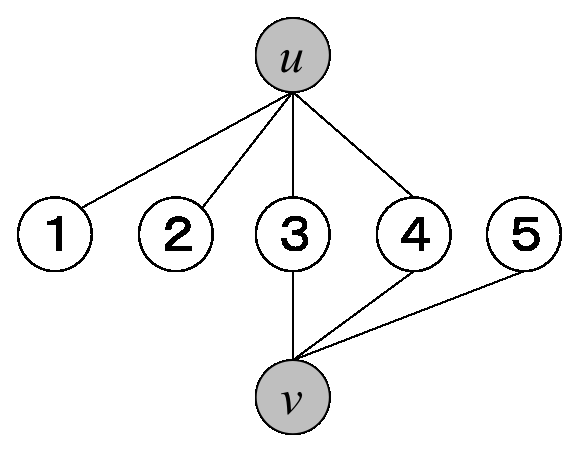
\includegraphics[scale=0.5]{./sim.eps}
\caption{頂点$u,v$の接続関係\label{fig:sim}}
\end{minipage}
\end{center}
\end{figure}

本コマンドでは、表\ref{tbl:simdef}に示されるように、6つの類似度を利用することができる。
類似度の選択は表中に示された\verb|sim=|パラメータを設定することによって行い、
\verb|th=|パラメータによって類似度の下限値を与える。

\begin{table}[htbp]
\begin{center}
\caption{グラフ$G=(V,E)$における節点$u,v$の類似度の定義\label{tbl:simdef}}
%{\small
\begin{tabular}{cllcc}
\hline
\# & 類似度&定義式&sim=パラメータ値&範囲 \\
\hline
1&recemblance    & $\frac{|N(u) \cap N(v)|}{|N(u) \cup N(v)|}$ & R & 0.0〜1.0\\
2&normalized PMI & $\log{\frac{P(u,v)}{P(u)P(v)}}/(-\log{P(u,v)})$ & P  & -1.0〜1.0\\
 &               & $=\frac{|V||N(u) \cap N(v)|}{|N(u)||N(v)|}/(-\log{\frac{|N(u) \cap N(v)|}{|V|}})$ & \\
3&intersection   & $|N(u) \cap N(v)|$ & T & 0〜\\
4&cosine         & $\frac{|N(u) \cap N(v)|}{\sqrt{|N(u)|}\sqrt{|N(v)|}}$ & C  & 0.0〜1.0\\
5&max-confidence & $\frac{|N(u) \cap N(v)|}{\max{(|N(u)|,|N(v)|)}}$ & S  & 0.0〜1.0\\
6&min-confidence & $\frac{|N(u) \cap N(v)|}{\min{(|N(u)|,|N(v)|)}}$ & s  & 0.0〜1.0\\
\hline
\end{tabular} 
\\
{\scriptsize
$N(u)$は頂点$u$に隣接する頂点集合を表す。
$P(u)$は頂点$u$に枝が張られる確率を表し、$P(u)=N(u)/|V|$である。
}
\end{center}
\end{table}

\subsection{例}
本コマンドの入力データである一般グラフは、表\ref{tbl:input}に示されるような、
枝データを節点ペアとして表したCSV形式で与える。
グラフは無向グラフとして扱われ、島が複数あってもよい。
枝を一つも持たない節点は、研磨の対象とならない(友達がいない)ために、節点データを別途入力することはない。
表\ref{tbl:input}のデータを視覚化したグラフを図\ref{fig:inputg}に示す。
以下では、このデータを使いデータ研磨の例を示していく。

\begin{table}[htbp]
\begin{center}
\caption{入力データ(枝データ)\label{tbl:input}}
\begin{tabular}{cc}
\hline
node1&node2 \\
\hline
a&b\\
a&c\\
a&e\\
b&c\\
b&e\\
b&g\\
c&d\\
c&g\\
d&e\\
e&f\\
\hline
\end{tabular} 
\end{center}
\end{table} 

簡単のために、類似度の定義をintersectionとしその下限値を2に設定したとしよう。
すなわち、隣接する節点で共通の節点数(共通する友達の数)が2以上である時に枝を張り、
そうでなければ枝を張らない。
例えば、図\ref{fig:ad}は、図\ref{fig:inputg}から節点$a,b$と連結のある節点を抜き出した部分グラフである。
2つの節点$e,c$を共通に持つため、研磨グラフにおいて、節点$a,b$に枝が張られる。
一方で節点$e,g$(図\ref{fig:eg})は、共通節点は節点$b$だけなので、研磨グラフにおいても枝は張られない。

\begin{figure}[htbp]
\begin{center}
\begin{tabular}{ccc}

\begin{minipage}{0.3\hsize}
\begin{center}
\includegraphics[scale=0.5]{./inputg.eps}
\caption{表\ref{tbl:input}のグラフデータを視覚化\label{fig:inputg}}
\end{center}
\end{minipage}

\begin{minipage}{0.2\hsize}
\begin{center}
\includegraphics[scale=0.5]{./ad.eps}
\caption{節点$a$と節点$d$の関係\label{fig:ad}}
\end{center}
\end{minipage}

\begin{minipage}{0.2\hsize}
\begin{center}
\includegraphics[scale=0.5]{./eg.eps}
\caption{節点$e$と節点$g$の関係\label{fig:eg}}
\end{center}
\end{minipage}

\end{tabular}
\end{center}
\end{figure}

図\ref{fig:ab2}は、節点$a,b$に関連する部分グラフである。
これまでの2つの例と異なる点は、節点$a,b$に直接の接続があることである。
このような場合、2つの考え方を取ることができる。
ひとつは、図\ref{fig:ab1}のように、直接の関係は考慮せず、あくまでも共通の友達関係だけを考慮する方法である。
もう一つの方法は、節点$a,b$をお互いに共通の友達と考え、架空の節点$a',b'$を追加し、$a,b$双方からの接続を仮定する。
よって、直接の接続がある場合、それだけで2人の友達を共通に持つと考える。

\begin{figure}[htbp]
\begin{center}
\begin{tabular}{ccc}

\begin{minipage}{0.3\hsize}
\begin{center}
\includegraphics[scale=0.5]{./ab2.eps}
\caption{節点$a$と節点$b$の関係\label{fig:ab2}}
\end{center}
\end{minipage}

\begin{minipage}{0.3\hsize}
\begin{center}
\includegraphics[scale=0.5]{./ab1.eps}
\caption{直接の接続を考慮しない例\label{fig:ab1}}
\end{center}
\end{minipage}

\begin{minipage}{0.3\hsize}
\begin{center}
\includegraphics[scale=0.5]{./ab3.eps}
\caption{直接の接続を考慮する例\label{fig:ab3}}
\end{center}
\end{minipage}

\end{tabular}
\end{center}
\end{figure}

以上のようにすべての節点ペアについて新たな接続関係を更新すると、
直接の関係を考慮しない場合は図\ref{fig:polished0}のような研磨グラフが得られ、
直接の関係を考慮する場合は図\ref{fig:polished2}のような研磨グラフが得られる。
そして、新たに得られたこれらの研磨グラフに繰り返しデータ研磨を付していくと、
3回でグラフ構造は変化しなくなり(収束し)、
図\ref{fig:polished1}と図\ref{fig:polished3}が得られる。
直接接続を考慮しない場合は、接続関係がすべて無くなる。
一方で直接接続を考慮する場合は、6つの節点$a,b,c,d,e,g$が互いに接続され、
極大クリークが形成される。
また節点$f$は$e$とのみ接続が残り、これも極大クリーク$e,f$を形成している。
なお、データ研磨を繰り返し適用すると、グラフ構造は安定してくるが、
収束しないケースもあることに注意する。

\begin{figure}[htbp]
\begin{center}
\begin{tabular}{cccc}

\begin{minipage}{0.25\hsize}
\begin{center}
\includegraphics[scale=0.5]{./polished0.eps}
\caption{直接考慮しない1回研磨グラフ\label{fig:polished0}}
\end{center}
\end{minipage}

\begin{minipage}{0.25\hsize}
\begin{center}
\includegraphics[scale=0.5]{./polished1.eps}
\caption{直接考慮しない3回研磨グラフ\label{fig:polished1}}
\end{center}
\end{minipage}

\begin{minipage}{0.25\hsize}
\begin{center}
\includegraphics[scale=0.5]{./polished2.eps}
\caption{直接考慮した1回研磨グラフ\label{fig:polished2}}
\end{center}
\end{minipage}

\begin{minipage}{0.25\hsize}
\begin{center}
\includegraphics[scale=0.5]{./polished3.eps}
\caption{直接考慮した3回研磨グラフ\label{fig:polished3}}
\end{center}
\end{minipage}

\end{tabular}
\end{center}
\end{figure}

以上は理解のし易さのために、共通する枝の数を類似度と定義してデータ研磨を行ったが、
グラフのサイズが大きくなると、思ったような研磨ができないことが多い。
隣接節点の数が増えるに伴って巨大な次数の頂点が発生し、関係が薄いにも
関わらず十分な数の共通接点を持つ節点ペアにも枝が張られてしまうからである。
%隣接節点の数が増えるに伴って、
%共通節点の数が相対的に低い(関係の薄い)節点ペアが出てくるが、
%共通節点数の下限値が固定されているため、そのような関係の薄い節点ペアにも枝が張られてしまうからである。
そこで、通常は、resemblanceを始めとした、相対的な共通性を評価できる類似度を使う。
類似度としてresenmblanceを用い、その下限値を0.4,0.5として収束するまで研磨したグラフを
図\ref{fig:resemblance04},\ref{fig:resemblance05}にそれぞれ示している。
また図\ref{fig:pmi02}は、類似度としてnormalized PMIを、下限値を0.2とした結果である。

\begin{figure}[htbp]
\begin{center}
\begin{tabular}{ccc}

\begin{minipage}{0.3\hsize}
\begin{center}
\includegraphics[scale=0.5]{./resemblance04.eps}
\caption{recemblance=0.4による研磨グラフ\label{fig:resemblance04}}
\end{center}
\end{minipage}

\begin{minipage}{0.3\hsize}
\begin{center}
\includegraphics[scale=0.5]{./resemblance05.eps}
\caption{recemblance=0.5による研磨グラフ\label{fig:resemblance05}}
\end{center}
\end{minipage}

\begin{minipage}{0.3\hsize}
\begin{center}
\includegraphics[scale=0.5]{./pmi02.eps}
\caption{normalized PIM=0.2による研磨グラフ\label{fig:pmi02}}
\end{center}
\end{minipage}

\end{tabular}
\end{center}
\end{figure}

なお、出力としては研磨グラフ以外にも表\ref{tbl:stat}に示されるような各種統計を出力することができる(\verb|log=|で指定したファイル)。

\begin{table}[htbp]
\begin{center}
\caption{ログに出力される各種統計\label{tbl:stat}}
%{\small
\begin{tabular}{ll}
\hline
key & 内容 \\
\hline
iter & データ研磨を適用した回数 \\
time & 実行時間\\
nSize0 & データ研磨前のグラフの節点数 \\
eSize0 & データ研磨前のグラフの枝数 \\
dens0  & データ研磨前の枝密度 \\
nSize\# & \#回目のデータ研磨後の節点数 \\
eSize\# & \#回目のデータ研磨後の枝数 \\
dens\#  & \#回目のデータ研磨後の枝密度 \\

\hline
\end{tabular} 
\end{center}
\end{table}


以下にデータ研磨の特徴をまとめておく。
\begin{itemize}
\item 共通する隣接節点の情報にしたがって枝を張り直す。
\item 6つの類似度を選ぶことができ、利用する類似度によって結果は異なってくる。
\item データ研磨を繰り返すことでグラフ構造は安定してくる(多くの場合は収束する)。
\item オリジナルのグラフに比べ極大クリークの数が劇的に少なくなる。
\item 類似度の下限値を低くすると、より大きな極大クリークが形成される。
\end{itemize}


\subsection{書式}
\begin{verbatim}
mpolishing.rb ei= ef= [ni=] [nf=] eo= [no=] [sim=R|P|C|s|S|T] th= [sup=] [-indirect] [iter=] [log=] [T=] [--help]

  ファイル名指定
  ei=    : 枝データファイル
  ef=    : 枝データ上の2つの節点項目名(省略時は"node1,node2")
  ni=    : 節点データファイル
  nf=    : 節点データ上の節点項目名(省略時は"node")
  eo=    : データ研磨後の枝データファイル
  no=    : データ研磨後の節点データファイル
  sim=   : 節点a,bと接続された枝集合を、それぞれA,Bとすると、節点a,bに枝を張るために用いる類似度。
           省略時はRが設定される。
             i: inclusion
             I: both-inclusion
             S: |A∩B|/max(|A|,|B|)
             s: |A∩B|/min(|A|,|B|)
             T (intersection): find pairs having common [threshld] items
             R (resemblance): find pairs s.t. |A\capB|/|A\cupB| >= [threshld]
             P (PMI): find pairs s.t. log (|A\capB|*|all| / (|A|*|B|)) >= [threshld]
             C (cosine distance): find pairs s.t. inner product of their normalized vectors >= [threshld]
  th=    : sim=で指定された類似度について、ここで指定された値以上の節点間に枝を張る。
  sup=   : 類似度計算において、|A∩B|>=supの条件を加える。省略すればsup=0。
  -indirect: 上記類似度計算における隣接節点集合から直接の関係を除外する。
             すなわち、A=A-b, B=B-a として類似度を計算する。
  iter=  : データ研磨の最大繰り返し数(デフォルト=30)
  log=   : パラメータの設定値や収束回数等をkey-value形式のCSVで保存するファイル名
  O=     : データ研磨過程のグラフを保存するディレクトリ名

  その他
  T= : ワークディレクトリ(default:/tmp)
  --help : ヘルプの表示
\end{verbatim}

\subsection{利用例}
\subsubsection*{Example 1: Basic Example}

Use resemblance(sim=R) as similarity measure, the polished graph is obtained by extending the branch at th=0.4.
The number of polishing iterations are converged 3 times as shown in \verb|log1.csv| (iter,4)。
The output result is shown in Figure \ref{fig:resemblance04}.


\begin{Verbatim}[baselinestretch=0.7,frame=single]
$ more dat1.csv
node1,node2
a,b
a,c
a,e
b,c
b,e
b,g
c,d
c,g
d,e
e,f
$ mpolishing.rb i=dat1.csv f=node1,node2 sim=R th=0.4 o=result1.csv log=log1.csv
#MSG# converting graph files into a pair of numbered nodes ...
input-file /tmp/__MTEMP_20042_70166767738540_2, output-file /tmp/__MTEMP_20042_70166767738
540_3
degree threshold: 
first & second scan end: /tmp/__MTEMP_20042_70166767738540_2
file read end: /tmp/__MTEMP_20042_70166767738540_2
iterative scan: #nodes=7, #edges = 20
forwardstar graph: /tmp/__MTEMP_20042_70166767738540_2 ,#nodes 7(7,7) ,#edges 20
#MSG# polishing iteration #0 (tra size=61
sspc_20140215 R -l 0 /tmp/__MTEMP_20042_70166767738540_3 0.4 /tmp/__MTEMP_20042_7016676773
8540_2
trsact: /tmp/__MTEMP_20042_70166767738540_3 ,#transactions 7 ,#items 7 ,size 27 extracted 
database: #transactions 7 ,#items 7 ,size 27
 output to: /tmp/__MTEMP_20042_70166767738540_2
separated at 0
11 pairs are found
0,1,2,4, :1.000000  (0)
0,1,2,4,6, :1.000000  (0)
0,1,2,3,6, :1.000000  (0)
2,3,4, :1.000000  (0)
0,1,3,4,5, :1.000000  (0)
4,5, :1.000000  (0)
1,2,6, :1.000000  (0)
come
input-file /tmp/__MTEMP_20042_70166767738540_2, output-file /tmp/__MTEMP_20042_70166767738
540_3
degree threshold: 
first & second scan end: /tmp/__MTEMP_20042_70166767738540_2
file read end: /tmp/__MTEMP_20042_70166767738540_2
iterative scan: #nodes=7, #edges = 22
forwardstar graph: /tmp/__MTEMP_20042_70166767738540_2 ,#nodes 7(7,7) ,#edges 22
#MSG# polishing iteration #1 (tra size=65
sspc_20140215 R -l 0 /tmp/__MTEMP_20042_70166767738540_3 0.4 /tmp/__MTEMP_20042_7016676773
8540_2
trsact: /tmp/__MTEMP_20042_70166767738540_3 ,#transactions 7 ,#items 7 ,size 29 extracted 
database: #transactions 7 ,#items 7 ,size 29
 output to: /tmp/__MTEMP_20042_70166767738540_2
separated at 0
11 pairs are found
0,1,2,3,4,6, :1.000000  (0)
0,1,2,4,6, :1.000000  (0)
0,1,2,4,6, :1.000000  (0)
0,3, :1.000000  (0)
0,1,2,4,5, :1.000000  (0)
4,5, :1.000000  (0)
0,1,2,6, :1.000000  (0)
come
input-file /tmp/__MTEMP_20042_70166767738540_2, output-file /tmp/__MTEMP_20042_70166767738
540_3
degree threshold: 
first & second scan end: /tmp/__MTEMP_20042_70166767738540_2
file read end: /tmp/__MTEMP_20042_70166767738540_2
iterative scan: #nodes=6, #edges = 22
forwardstar graph: /tmp/__MTEMP_20042_70166767738540_2 ,#nodes 7(7,7) ,#edges 22
#MSG# polishing iteration #2 (tra size=63
sspc_20140215 R -l 0 /tmp/__MTEMP_20042_70166767738540_3 0.4 /tmp/__MTEMP_20042_7016676773
8540_2
trsact: /tmp/__MTEMP_20042_70166767738540_3 ,#transactions 7 ,#items 7 ,size 28 extracted 
database: #transactions 7 ,#items 7 ,size 28
 output to: /tmp/__MTEMP_20042_70166767738540_2
separated at 0
10 pairs are found
0,1,2,4,6, :1.000000  (0)
0,1,2,4,6, :1.000000  (0)
0,1,2,4,6, :1.000000  (0)
 :1.000000  (0)
0,1,2,4,5,6, :1.000000  (0)
4,5, :1.000000  (0)
0,1,2,4,6, :1.000000  (0)
come
input-file /tmp/__MTEMP_20042_70166767738540_2, output-file /tmp/__MTEMP_20042_70166767738
540_3
degree threshold: 
first & second scan end: /tmp/__MTEMP_20042_70166767738540_2
file read end: /tmp/__MTEMP_20042_70166767738540_2
iterative scan: #nodes=5, #edges = 20
forwardstar graph: /tmp/__MTEMP_20042_70166767738540_2 ,#nodes 7(7,7) ,#edges 20
#MSG# polishing iteration #3 (tra size=57
sspc_20140215 R -l 0 /tmp/__MTEMP_20042_70166767738540_3 0.4 /tmp/__MTEMP_20042_7016676773
8540_2
trsact: /tmp/__MTEMP_20042_70166767738540_3 ,#transactions 7 ,#items 7 ,size 25 extracted 
database: #transactions 7 ,#items 7 ,size 25
 output to: /tmp/__MTEMP_20042_70166767738540_2
separated at 0
10 pairs are found
0,1,2,4,6, :1.000000  (0)
0,1,2,4,6, :1.000000  (0)
0,1,2,4,6, :1.000000  (0)
 :1.000000  (0)
0,1,2,4,6, :1.000000  (0)
 :1.000000  (0)
0,1,2,4,6, :1.000000  (0)
come
input-file /tmp/__MTEMP_20042_70166767738540_2, output-file /tmp/__MTEMP_20042_70166767738
540_3
degree threshold: 
first & second scan end: /tmp/__MTEMP_20042_70166767738540_2
file read end: /tmp/__MTEMP_20042_70166767738540_2
iterative scan: #nodes=5, #edges = 20
forwardstar graph: /tmp/__MTEMP_20042_70166767738540_2 ,#nodes 7(7,7) ,#edges 20
#MSG# converting the numbered nodes into original name ...
#END# /Users/stephane/.rvm/rubies/ruby-1.9.3-p448/bin/mpolishing.rb i=dat1.csv f=node1,nod
e2 sim=R th=0.4 o=result1.csv log=log1.csv
$ more result1.csv
node1,node2
a,b
a,c
a,e
a,g
b,c
b,e
b,g
c,e
c,g
e,g
$ more log1.csv
key,value
i=,dat1.csv
f=,"node1,node2"
sim=,R
th=,0.4
o=,result1.csv
log=,log1.csv
-int,false
-indirect,false
iter,4
time,0.113653
nSize0,7
eSize0,10
dens0,0.4761904762
nSize1,7
eSize1,11
dens1,0.5238095238
nSize2,6
eSize2,11
dens2,0.7333333333
nSize3,5
eSize3,10
dens3,1
nSize4,5
eSize4,10
dens4,1
\end{Verbatim}
\subsubsection*{Example 2: Polishing by PMI}

Use normalized PMI(sim=P) as similarity measure, the polished graph is obtained by extending the branch at th=0.2.
The output result is shown in Figure \ref{fig:pmi02}.



\begin{Verbatim}[baselinestretch=0.7,frame=single]
$ mpolishing.rb i=dat1.csv f=node1,node2 sim=P th=0.2 o=result2.csv
#MSG# converting graph files into a pair of numbered nodes ...
input-file /tmp/__MTEMP_20101_70350905868560_2, output-file /tmp/__MTEMP_20101_70350905868
560_3
degree threshold: 
first & second scan end: /tmp/__MTEMP_20101_70350905868560_2
file read end: /tmp/__MTEMP_20101_70350905868560_2
iterative scan: #nodes=7, #edges = 20
forwardstar graph: /tmp/__MTEMP_20101_70350905868560_2 ,#nodes 7(7,7) ,#edges 20
#MSG# polishing iteration #0 (tra size=61
sspc_20140215 P -l 0 /tmp/__MTEMP_20101_70350905868560_3 0.2 /tmp/__MTEMP_20101_7035090586
8560_2
trsact: /tmp/__MTEMP_20101_70350905868560_3 ,#transactions 7 ,#items 7 ,size 27 extracted 
database: #transactions 7 ,#items 7 ,size 27
 output to: /tmp/__MTEMP_20101_70350905868560_2
separated at 0
5 pairs are found
0,1,2,4, :1.000000  (0)
0,1,2,4,6, :1.000000  (0)
0,1,2,3,6, :1.000000  (0)
2,3,4, :1.000000  (0)
0,1,3,4,5, :1.000000  (0)
4,5, :1.000000  (0)
1,2,6, :1.000000  (0)
come
input-file /tmp/__MTEMP_20101_70350905868560_2, output-file /tmp/__MTEMP_20101_70350905868
560_3
degree threshold: 
first & second scan end: /tmp/__MTEMP_20101_70350905868560_2
file read end: /tmp/__MTEMP_20101_70350905868560_2
iterative scan: #nodes=6, #edges = 10
forwardstar graph: /tmp/__MTEMP_20101_70350905868560_2 ,#nodes 7(7,7) ,#edges 10
#MSG# polishing iteration #1 (tra size=39
sspc_20140215 P -l 0 /tmp/__MTEMP_20101_70350905868560_3 0.2 /tmp/__MTEMP_20101_7035090586
8560_2
trsact: /tmp/__MTEMP_20101_70350905868560_3 ,#transactions 7 ,#items 7 ,size 16 extracted 
database: #transactions 7 ,#items 7 ,size 16
 output to: /tmp/__MTEMP_20101_70350905868560_2
separated at 0
5 pairs are found
0,1, :1.000000  (0)
0,1,2,6, :1.000000  (0)
1,2,6, :1.000000  (0)
 :1.000000  (0)
4,5, :1.000000  (0)
4,5, :1.000000  (0)
1,2,6, :1.000000  (0)
come
input-file /tmp/__MTEMP_20101_70350905868560_2, output-file /tmp/__MTEMP_20101_70350905868
560_3
degree threshold: 
first & second scan end: /tmp/__MTEMP_20101_70350905868560_2
file read end: /tmp/__MTEMP_20101_70350905868560_2
iterative scan: #nodes=6, #edges = 10
forwardstar graph: /tmp/__MTEMP_20101_70350905868560_2 ,#nodes 7(7,7) ,#edges 10
#MSG# converting the numbered nodes into original name ...
#END# /Users/stephane/.rvm/rubies/ruby-1.9.3-p448/bin/mpolishing.rb i=dat1.csv f=node1,nod
e2 sim=P th=0.2 o=result2.csv
$ more result2.csv
node1,node2
a,b
b,c
b,g
c,g
e,f
\end{Verbatim}
\subsubsection*{Example 3: Polish once at intersection}

Based on the explanation in the previous example. Use intersection(sim=T) as similarity measure, consider cases with 2 or more (th=2) branch extension with direct connection. Polish graph with 1 iteration (iter=1).
The output result is shown in Figure \ref{fig:polished2}.



\begin{Verbatim}[baselinestretch=0.7,frame=single]
$ mpolishing.rb i=dat1.csv f=node1,node2 sim=T th=2 iter=1 o=result3.csv
#MSG# converting graph files into a pair of numbered nodes ...
input-file /tmp/__MTEMP_20151_70168512314200_2, output-file /tmp/__MTEMP_20151_70168512314
200_3
degree threshold: 
first & second scan end: /tmp/__MTEMP_20151_70168512314200_2
file read end: /tmp/__MTEMP_20151_70168512314200_2
iterative scan: #nodes=7, #edges = 20
forwardstar graph: /tmp/__MTEMP_20151_70168512314200_2 ,#nodes 7(7,7) ,#edges 20
#MSG# polishing iteration #0 (tra size=61
sspc_20140215 T -l 0 /tmp/__MTEMP_20151_70168512314200_3 2.0 /tmp/__MTEMP_20151_7016851231
4200_2
trsact: /tmp/__MTEMP_20151_70168512314200_3 ,#transactions 7 ,#items 7 ,size 27 extracted 
database: #transactions 7 ,#items 7 ,size 27
 output to: /tmp/__MTEMP_20151_70168512314200_2
separated at 0
14 pairs are found
0,1,2,4, :1.000000  (0)
0,1,2,4,6, :1.000000  (0)
0,1,2,3,6, :1.000000  (0)
2,3,4, :1.000000  (0)
0,1,3,4,5, :1.000000  (0)
4,5, :1.000000  (0)
1,2,6, :1.000000  (0)
come
input-file /tmp/__MTEMP_20151_70168512314200_2, output-file /tmp/__MTEMP_20151_70168512314
200_3
degree threshold: 
first & second scan end: /tmp/__MTEMP_20151_70168512314200_2
file read end: /tmp/__MTEMP_20151_70168512314200_2
iterative scan: #nodes=7, #edges = 28
forwardstar graph: /tmp/__MTEMP_20151_70168512314200_2 ,#nodes 7(7,7) ,#edges 28
#MSG# converting the numbered nodes into original name ...
#END# /Users/stephane/.rvm/rubies/ruby-1.9.3-p448/bin/mpolishing.rb i=dat1.csv f=node1,nod
e2 sim=T th=2 iter=1 o=result3.csv
$ more result3.csv
node1,node2
a,b
a,c
a,d
a,e
a,g
b,c
b,d
b,e
b,g
c,d
c,e
c,g
d,e
e,f
\end{Verbatim}
\subsubsection*{Example 4: Exclude direct connection}

When \verb|-indirect| is specified, direct connection is ignored when calculating degree of similarity.
The output graph is shown in Figure \ref{fig:polished1}, to remove all branches, branch data is not returned after polishing.


\begin{Verbatim}[baselinestretch=0.7,frame=single]
$ mpolishing.rb i=dat1.csv f=node1,node2 sim=T th=2 o=result4.csv -indirect
#MSG# converting graph files into a pair of numbered nodes ...
input-file /tmp/__MTEMP_20194_70296082596580_2, output-file /tmp/__MTEMP_20194_70296082596
580_3
degree threshold: 
first & second scan end: /tmp/__MTEMP_20194_70296082596580_2
file read end: /tmp/__MTEMP_20194_70296082596580_2
iterative scan: #nodes=7, #edges = 20
forwardstar graph: /tmp/__MTEMP_20194_70296082596580_2 ,#nodes 7(7,7) ,#edges 20
#MSG# polishing iteration #0 (tra size=47
sspc_20140215 T -l 0 /tmp/__MTEMP_20194_70296082596580_3 2.0 /tmp/__MTEMP_20194_7029608259
6580_2
trsact: /tmp/__MTEMP_20194_70296082596580_3 ,#transactions 7 ,#items 7 ,size 20 extracted 
database: #transactions 7 ,#items 7 ,size 20
 output to: /tmp/__MTEMP_20194_70296082596580_2
separated at 0
6 pairs are found
1,2,4, :1.000000  (0)
0,2,4,6, :1.000000  (0)
0,1,3,6, :1.000000  (0)
2,4, :1.000000  (0)
0,1,3,5, :1.000000  (0)
4, :1.000000  (0)
1,2, :1.000000  (0)
come
input-file /tmp/__MTEMP_20194_70296082596580_2, output-file /tmp/__MTEMP_20194_70296082596
580_3
degree threshold: 
first & second scan end: /tmp/__MTEMP_20194_70296082596580_2
file read end: /tmp/__MTEMP_20194_70296082596580_2
iterative scan: #nodes=6, #edges = 12
forwardstar graph: /tmp/__MTEMP_20194_70296082596580_2 ,#nodes 7(7,7) ,#edges 12
#MSG# polishing iteration #1 (tra size=31
sspc_20140215 T -l 0 /tmp/__MTEMP_20194_70296082596580_3 2.0 /tmp/__MTEMP_20194_7029608259
6580_2
trsact: /tmp/__MTEMP_20194_70296082596580_3 ,#transactions 7 ,#items 7 ,size 12 extracted 
database: #transactions 7 ,#items 7 ,size 12
 output to: /tmp/__MTEMP_20194_70296082596580_2
separated at 0
0 pairs are found
1,3,6, :1.000000  (0)
0,2,3, :1.000000  (0)
1,4, :1.000000  (0)
0,1, :1.000000  (0)
2, :1.000000  (0)
 :1.000000  (0)
0, :1.000000  (0)
come
input-file /tmp/__MTEMP_20194_70296082596580_2, output-file /tmp/__MTEMP_20194_70296082596
580_3
degree threshold: 
first & second scan end: /tmp/__MTEMP_20194_70296082596580_2
file read end: /tmp/__MTEMP_20194_70296082596580_2
iterative scan: #nodes=0, #edges = 0
forwardstar graph: /tmp/__MTEMP_20194_70296082596580_2 ,#nodes 0(0,0) ,#edges 0
#MSG# polishing iteration #2 (tra size=6
sspc_20140215 T -l 0 /tmp/__MTEMP_20194_70296082596580_3 2.0 /tmp/__MTEMP_20194_7029608259
6580_2
trsact: /tmp/__MTEMP_20194_70296082596580_3 ,#transactions 2 ,#items 4 ,size 1 extracted d
atabase: #transactions 2 ,#items 4 ,size 1
 output to: /tmp/__MTEMP_20194_70296082596580_2
separated at 0
0 pairs are found
 :1.000000  (0)
3, :1.000000  (0)
come
input-file /tmp/__MTEMP_20194_70296082596580_2, output-file /tmp/__MTEMP_20194_70296082596
580_3
degree threshold: 
first & second scan end: /tmp/__MTEMP_20194_70296082596580_2
file read end: /tmp/__MTEMP_20194_70296082596580_2
iterative scan: #nodes=0, #edges = 0
forwardstar graph: /tmp/__MTEMP_20194_70296082596580_2 ,#nodes 0(0,0) ,#edges 0
#MSG# converting the numbered nodes into original name ...
#END# /Users/stephane/.rvm/rubies/ruby-1.9.3-p448/bin/mpolishing.rb i=dat1.csv f=node1,nod
e2 sim=T th=2 o=result4.csv -indirect
$ more result4.csv
node1,node2
\end{Verbatim}



